\section{Setup at Hj{\o}rring Library}

On the last weeks of the project, the group finally decided to show up at Hj{\o}rring Library to setup the project in order to test it and make the final arrangements. The project itself requires a canvas, some illumination from LEDs, an infrared camera and a projector.

\begin{itemize}
\item LEDs strips

The first step on the construction of the Canvas was to position two LEDs strips in order to get the desired illumination for the infrared camera. As the placement of this project is a corridor divided by a red shelve that crosses the whole library, it was decided to add one strip on the lower part of this shelve and another LED stripes on the background covered by the canvas (see picture \ref{fig:LEDsPosition}).

\begin{figure}[htbp] 
\centering 
\includegraphics[width=0.5\textwidth]{Pictures/Design/stand1.png} 
\caption{Light as captured by a camera} 
\label{fig:LEDsPosition} 
\end{figure}

The construction of these LEDs stripes was made as simple as possible in order to lighten the weight. So finally the stripes were tapped to the shelves with duct tape. The solutions can be seen on Fig. \ref{fig:RealLEDs} and \ref{fig:RealRedLEDs}.

\begin{figure}[htbp] \centering
\begin{minipage}[b]{0.45\textwidth} \centering
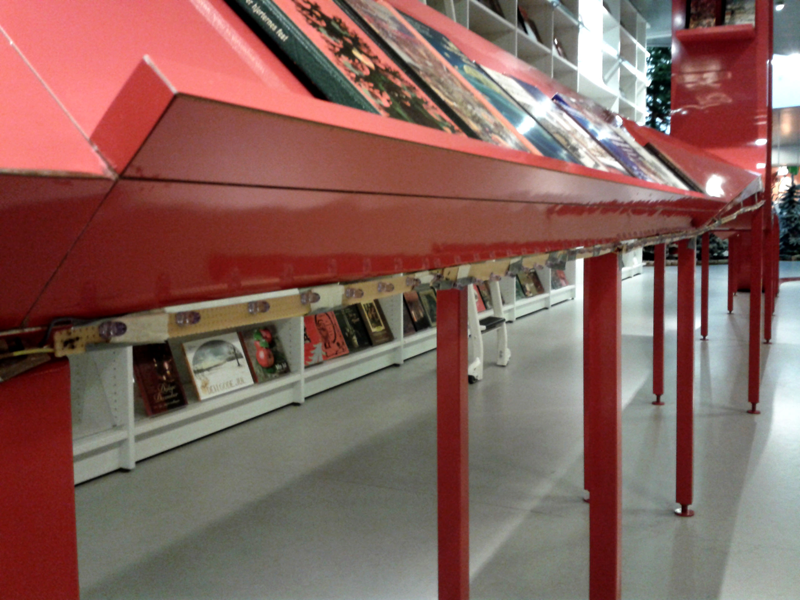
\includegraphics[width=1.00\textwidth]{Pictures/Design/LEDRedShelve.png}
\caption{LED stripes construction}
\label{fig:RealRedLEDs}
\end{minipage} \hfill
\begin{minipage}[b]{0.45\textwidth} \centering
\includegraphics[width=1.00\textwidth]{Pictures/Design/LEDShelve.png} 
\caption{LED stripes construction}
\label{fig:RealLEDs}
\end{minipage} \hfill
\end{figure}

\item Building the Canvas

For the projection it was decided to use a sheet to cover the 
\begin{figure}[htbp] 
\centering 
\includegraphics[width=0.5\textwidth]{Pictures/Design/stand2.png} 
\caption{Light as captured by a camera} 
\label{fig:CanvasPosition} 
\end{figure}

\end{itemize}